\documentclass[11pt]{examdesign}
\usepackage{amsmath}
\usepackage{enumitem}
\usepackage{amsfonts}
\usepackage{pgfplots}
\usepackage{pifont}
\usepackage{graphicx}
\usepackage{fancyhdr}
\usepackage{cancel}
\usepackage[american]{circuitikz}

\SectionFont{\large\sffamily}
\Fullpages
\ContinuousNumbering
\usepackage{ulem}
\ProportionalBlanks{2}


\DefineAnswerWrapper{}{}
\NumberOfVersions{1}
%\IncludeFromFile{foobar.tex}
\examname{\Large{Graphing Motion}}
\class {\Large Physics}

\def \namedata {Name: \hrulefill\\ 
	Date: \hrulefill \\
	Period: \hrulefill \\
	Primary Peer Reviewer: \hrulefill 
	\\
			\begin{tabular}{| p{1cm} | p{1cm} | p{1 cm} | p{1cm} |}
	\hline
		+1 & 0 & -1 & $\Sigma$ 
		\\
		\hline
		& & & \vspace{.5cm}
		\\ \hline
	
	\end{tabular}
	\\
 \vspace{-.6in}
	
}




\begin{document}




\begin{multiplechoice} [title={Multiple Choice},
	rearrange=no]
	\vspace{0.1in}
\textbf{The following information applies to questions 1-3:}
	
	\begin{center}
	
	\vspace{0.1in}
	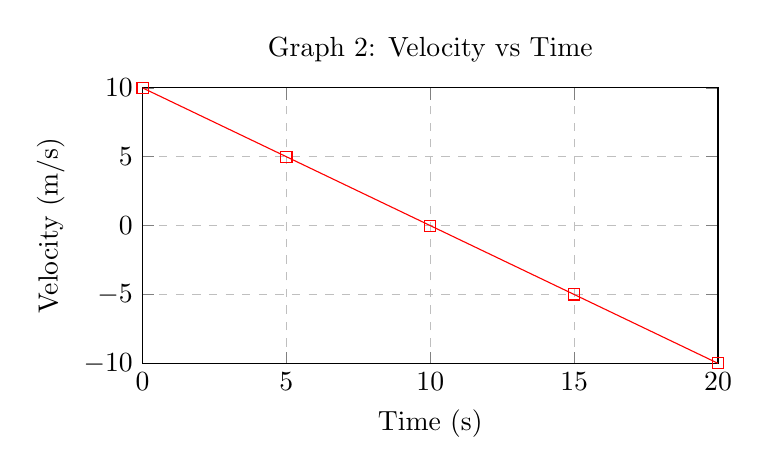
\begin{tikzpicture}
	\begin{axis}[
	title={Graph 2: Velocity vs Time},
	xlabel={Time (s)},
	ylabel={Velocity (m/s)},
	xmin=0, xmax=20,
	ymin=-10, ymax=10,
	xtick={0,5,10,15,20},
	ytick={-10,-5,0,5,10,15},
	ymajorgrids=true,
	xmajorgrids=true,
	grid style=dashed,
	legend pos=south east,
	height=2in,
	width=3.5in
	]
	
	\addplot[
	color=red,
	mark=square,
	]
	coordinates {
		(0,10)(5,5)(10,0)(15,-5)(20,-10)};

	

	
	
	\end{axis}
	\end{tikzpicture}
\end{center}
	\vspace{-0.25in}
	
	\begin{question}
	
	What is the speed of the object from 0-10 seconds?
	 \choice {0.5 m/s}
	 \choice {1.5 m/s}
	 \choice [!]{2 m/s}
	 \choice {20 m/s}
	\end{question}


\begin{question}
	During what time interval is this object stopped?
	\choice {0 seconds to 10 seconds}
	\choice [!]{10 seconds to 15 seconds}
	\choice {15 seconds to 20 seconds}
	\choice {The object is stopped only at 0 seconds.}
\end{question}

	\begin{question}
	Which of the following descriptions would best describe this graph?
	\choice [!]{An athlete runs 20 meters, stops, then begins to walk back to where he started.}
	\choice {A car accelerates, drives at a constant speed, then begins to slow down.}
	\choice {A man climbs a ladder, stands at the top, then falls off.}
	\choice {A marble rolls down a ramp, accelerating as it travels.}
\end{question}


	\begin{question}
	The area under a velocity-time graph is best described as -
	\choice [!]{Distance Traveled}
	\choice {Change in Velocity}
	\choice {Acceleration}
	\choice {Time}
\end{question}










\end{multiplechoice}

\begin{multiplechoice} [title={Multiple Correct Multiple Choice},
	rearrange=no]
	\textit{For the following question, \textbf{choose two} correct answers.  No credit will be given for incorrect or partially correct answers.  Mark \textbf{both} answers clearly.} 


	\begin{question}
		
		Which of the following graphs would represent an object traveling at a constant speed?
	\vspace{0.2in}
	
			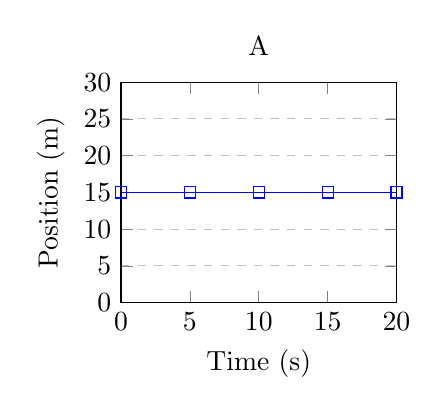
\begin{tikzpicture}
			\begin{axis}[
			title={A},
			xlabel={Time (s)},
			ylabel={Position (m)},
			xmin=0, xmax=20,
			ymin=0, ymax=30,
			xtick={0,5,10,15,20},
			ytick={0,5,10,15,20,25,30},
			ymajorgrids=true,
			grid style=dashed,
			legend pos=south east,
			width=2in
			]
			
			\addplot[
			color=blue,
			mark=square,
			]
			coordinates {
				(0,15)(5,15)(10,15)(15,15)(20,15)};
			\end{axis}
			\end{tikzpicture} \hspace{0.5in}%
			%
				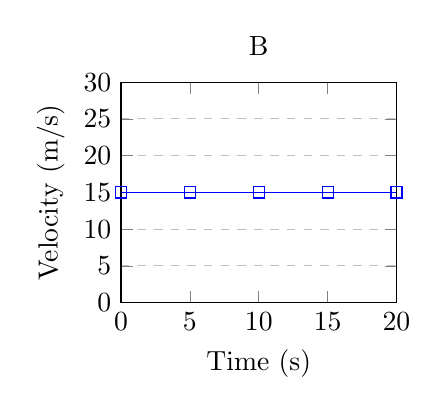
\begin{tikzpicture}
			\begin{axis}[
			title={B},
			xlabel={Time (s)},
			ylabel={Velocity (m/s)},
			xmin=0, xmax=20,
			ymin=0, ymax=30,
			xtick={0,5,10,15,20},
			ytick={0,5,10,15,20,25,30},
			ymajorgrids=true,
			grid style=dashed,
			legend pos=south east,
			width=2in
			]
			
			\addplot[
			color=blue,
			mark=square,
			]
			coordinates {
				(0,15)(5,15)(10,15)(15,15)(20,15)};
			\end{axis}
			\end{tikzpicture}
			
				\vspace{0.2in}
			
				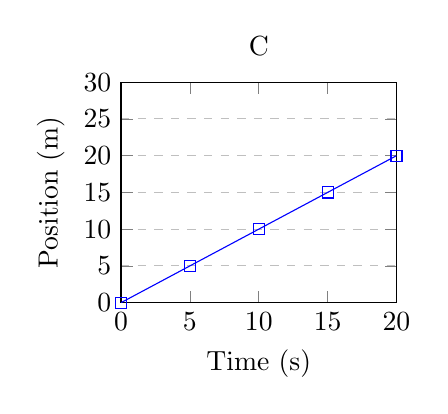
\begin{tikzpicture}
			\begin{axis}[
			title={C},
			xlabel={Time (s)},
			ylabel={Position (m)},
			xmin=0, xmax=20,
			ymin=0, ymax=30,
			xtick={0,5,10,15,20},
			ytick={0,5,10,15,20,25,30},
			ymajorgrids=true,
			grid style=dashed,
			legend pos=south east,
			width=2in
			]
			
			\addplot[
			color=blue,
			mark=square,
			]
			coordinates {
				(0,0)(5,5)(10,10)(15,15)(20,20)};
			\end{axis}
			\end{tikzpicture} \hspace{0.5in}%
			%
				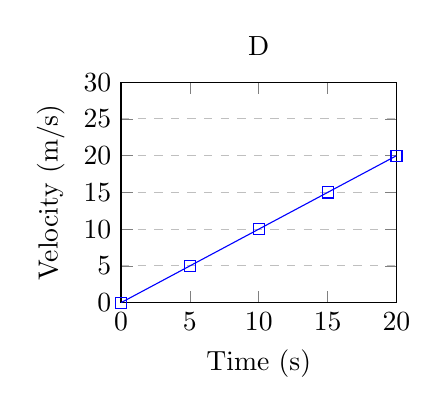
\begin{tikzpicture}
			\begin{axis}[
			title={D},
			xlabel={Time (s)},
			ylabel={Velocity (m/s)},
			xmin=0, xmax=20,
			ymin=0, ymax=30,
			xtick={0,5,10,15,20},
			ytick={0,5,10,15,20,25,30},
			ymajorgrids=true,
			grid style=dashed,
			legend pos=south east,
			width=2in
			]
			
			\addplot[
			color=blue,
			mark=square,
			]
			coordinates {
				(0,0)(5,5)(10,10)(15,15)(20,20)};
			\end{axis}
			\end{tikzpicture}
	
	\end{question}
	
	\begin{question}
		Which of the following can be determined from the following graph?
		\begin{center}
					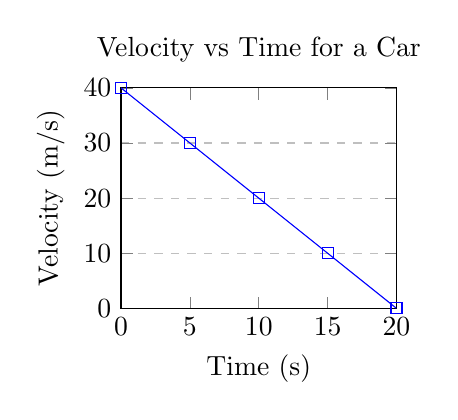
\begin{tikzpicture}
	\begin{axis}[
	title={Velocity vs Time for a Car},
	xlabel={Time (s)},
	ylabel={Velocity (m/s)},
	xmin=0, xmax=20,
	ymin=0, ymax=40,
	xtick={0,5,10,15,20},
	ytick={0,10,20,30,40},
	ymajorgrids=true,
	grid style=dashed,
	legend pos=south east,
	width=2in
	]
	
	\addplot[
	color=blue,
	mark=square,
	]
	coordinates {
		(0,40)(5,30)(10,20)(15,10)(20,0)};
	\end{axis}
	\end{tikzpicture}
\end{center}
		\choice[!]{The acceleration of the object is $-2 m/s^2$}
		\choice{The acceleration of the object is increasing.}
		\choice{The object is traveling backward.}
		\choice[!]{The distance the object travels is 400 m.}
		\choice{The speed of the object is constant.}
		
	\end{question}


\end{multiplechoice}

\pagebreak
\begin{shortanswer}[title={Free Response},
	rearrange=no]

\begin{question}
Sketch a Position vs. Time graph for:
\begin{enumerate}
	\item An object at rest.
	\vspace{0.75 in}
	\item An object moving in a positive direction with a constant speed.
	\vspace{0.75 in}
	\item An object moving in a negative direction with a constant speed.
	\vspace{0.75 in}
	\item An object that is accelerating in a positive direction, starting from rest.
	\vspace{0.75 in}
\end{enumerate}

\end{question}




\begin{question}

	Sketch a \textbf{Velocity-Time} graph for the following situation:
	A man is driving at a constant speed when he sees that his odometer is about to hit 100,000 miles.  He slows down and stops so that he can take out his phone to record the event.  He accelerates to the speed limit, and continues on at a constant speed.  He then realizes that he forgot to hit the record button. He slows down, then reverses the car to make his odometer run backward, stops, then drives forward again as he records the event.  
	
\end{question}

	\end{shortanswer}



\end{document}


